\documentclass{article} % For LaTeX2e
\usepackage{nips14submit_e,times}
\usepackage{amsmath}
\usepackage{amsthm}
\usepackage{amssymb}
\usepackage{mathtools}
\usepackage{hyperref}
\usepackage{url}
\usepackage{algorithm}
\usepackage[noend]{algpseudocode}
%\documentstyle[nips14submit_09,times,art10]{article} % For LaTeX 2.09

\usepackage{mathrsfs}
\usepackage{graphicx}
\usepackage{caption}
\usepackage{subcaption}

\def\eQb#1\eQe{\begin{eqnarray*}#1\end{eqnarray*}}
\def\eQnb#1\eQne{\begin{eqnarray}#1\end{eqnarray}}
\providecommand{\e}[1]{\ensuremath{\times 10^{#1}}}
\providecommand{\pb}[0]{\pagebreak}


\def\Qb#1\Qe{\begin{question}#1\end{question}}
\def\Sb#1\Se{\begin{solution}#1\end{solution}}

\newenvironment{claim}[1]{\par\noindent\underline{Claim:}\space#1}{}
\newtheoremstyle{quest}{\topsep}{\topsep}{}{}{\bfseries}{}{ }{\thmname{#1}\thmnote{ #3}.}
\theoremstyle{quest}
\newtheorem*{definition}{Definition}
\newtheorem*{theorem}{Theorem}
\newtheorem*{lemma}{Lemma}
\newtheorem*{question}{Question}
\newtheorem*{preposition}{Preposition}
\newtheorem*{exercise}{Exercise}
\newtheorem*{challengeproblem}{Challenge Problem}
\newtheorem*{solution}{Solution}
\newtheorem*{remark}{Remark}
\usepackage{verbatimbox}
\usepackage{listings}

\title{Real Variables: \\
Problem Set VIII}


\author{
Youngduck Choi \\
Courant Institute of Mathematical Sciences \\
New York University \\
\texttt{yc1104@nyu.edu} \\
}


% The \author macro works with any number of authors. There are two commands
% used to separate the names and addresses of multiple authors: \And and \AND.
%
% Using \And between authors leaves it to \LaTeX{} to determine where to break
% the lines. Using \AND forces a linebreak at that point. So, if \LaTeX{}
% puts 3 of 4 authors names on the first line, and the last on the second
% line, try using \AND instead of \And before the third author name.

\newcommand{\fix}{\marginpar{FIX}}
\newcommand{\new}{\marginpar{NEW}}

\nipsfinalcopy % Uncomment for camera-ready version

\begin{document}


\maketitle

\begin{abstract}
This work contains solutions to the problem set 
VIII of Real Variables 2015 at NYU.
\end{abstract}

\section{Solutions}

\begin{question}[1. Royden 11-30]
\hfill
\begin{figure}[h!]
  \centering
    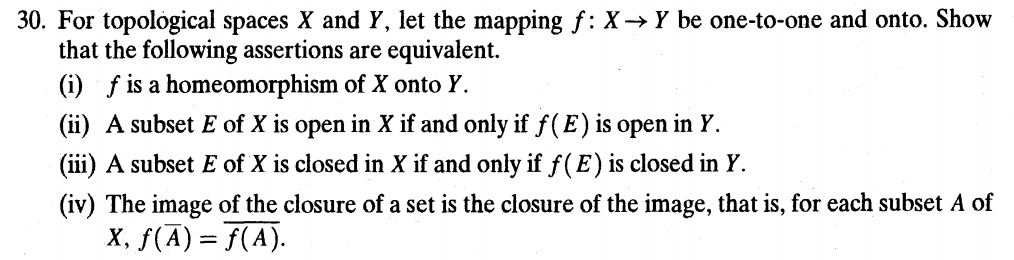
\includegraphics[width=1\textwidth]{11-30}
\end{figure}
\end{question}
\begin{solution}
Assume (i). Let $E$ be a subset of $X$. 
Assume that $E$ is open in $X$. As $f^{-1}$ is continuous, $f(E)$
is open. Conversely, assume that $f(E)$ is open. as $f$ is continuous,
$E$ is open in $X$. Therefore, (ii) holds.
Assume that (ii) holds. Then, for
any open set $O$ in $X$, $f(O)$ is open. As $f = {f^{-1}}^{-1}$,
$f^{-1}$ is continuous. 
Let $O$ be an open set in $Y$. As $f$ is surjective, there exists 
a subset $E$ of $X$ that $f(E) = O$. By (ii), $E$ is open. Hence,
$f^{-1}(O)$ is open. Hence $f$ is continuous. $f$ is a homeomorphism. 
Therefore, (i) and (ii) are equivalent.  

\bigskip

Assume (ii), and let $E$ be a subset of $X$. $E$ being closed is 
equivalent to $X \setminus E$ being open. By(ii), it is
equivalent to  $f(X\setminus E)$ being open. Since $f$ is injective, 
$f(X\setminus E) = f(X) \setminus E$. Again, as $f$ is surjective,
we have $f(X) =Y$ and it follows that $Y \setminus f(E)$ is open.
This is again equivalent to $f(E)$ being closed. Hence (ii) and (iii)
are equivalent. 
 
\bigskip

So far, we have shown that (i), (ii), and (iii) are equivalent. We now 
show that (i) implies (iv) and (iv) implies (iii). 
Assume (i). We claim that $f(\bar{A}) \subseteq \overline{f(A)}$. Let
$y \in f(\bar{A})$. Then, as $f$ is bijective, there exists 
an unique $x \in \bar{A}$, such that
$f(x) = y$. Since $f$ is homeomorphic, it is continuous. 
By continuity of $f$ at $x$, for any neighborhood $O$
of $y$, there exists a neighborhood $U$ of $x$, such that $f(U) \subseteq 
O$. As $x \in \bar{A}$, $U \cap A \neq \emptyset$, and $f(U) \cap f(A) 
\neq \emptyset$. Since $f(U) \subseteq O$, $f(A) \cap O \neq \emptyset$. 
Hence, $y \in \overline{f(A)}$. We now claim that
$\overline{f(A)} \subseteq f(\bar{A})$. Let $x \in \overline{f(A)}$.
As $f^{-1}$ is bijective, there exists an unique $y \in X$ such that
$y = f^{-1}(x)$ By the continuity of $f^{-1}$ at $x$, for any neighborhood 
O of $y$, there exists a neighborhood $U$ of $x$ such that $f^{-1}(U)
\subseteq O$. As $x \in \overline{f(A)}$, $U \cap f(A) \neq \emptyset$,
and $f^{-1}(U) \cap A \neq \emptyset$. Since $f^{-1}(U) \subseteq
O$, we have $O \cap A \neq \emptyset$. Hence, $y \in \overline{A}$. 
Hence, $x \in f(\overline{A})$. Therefore, we have shown that
$f(\bar{A}) = \overline{f(A)}$. 

\smallskip

Assume (iv). Let $E$ be a subset of $X$. Assume that $E$ is closed in $X$.
Then, $E = \overline{E}$. Consequently, by (iv), it follows that $f(E) = f(
\overline{E}) = \overline{f(E)}$. Since, $f(E) = \overline{f(E)}$, 
$f(E)$ is closed.  Now, assume that $f(E)$ is closed. Then, by (iv), 
it follows that $f(E) = \overline{f(E)} = f(\overline{E})$. Since $f$
is injective, $E = \overline{E}$ holds. Therefore, (iv) implies (iii). 

\bigskip

We have shown that all four statements are equivalent. \hfill $\qed$
\end{solution}

\bigskip

\begin{question}[2. Royden 11-34]
\hfill
\begin{figure}[h!]
  \centering
    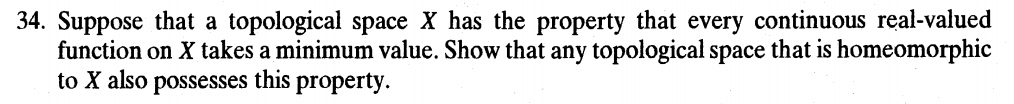
\includegraphics[width=1\textwidth]{11-34}
\end{figure}
\end{question}
\begin{solution}
Let $Y$ be a topological space that is homeomorphic to $X$. 
Let $g$ be a continuous real-valued function, defined on $Y$.
As $X$ and $Y$ are homeomorhpic, there exists a continuous bijection
from $X$ to $Y$, which we denote as $\phi$. Observe that 
$g \circ \phi$ is a real-valued function, defined on $X$. Since $\phi$
and $g$ are continuous, and composition of continuous maps is continuous,
we have $g \circ \phi$ is continuous on $X$. Therefore, by the given, 
$g \circ \phi(X)$ attains a minimum value. Since $\phi(X) = Y$, we have
$g \circ \phi(X) = g(Y)$. Hence, $g(Y)$ attains a minimum value. As $g$
was considered to be an arbitrary, continuous function,
all continuous function on $Y$ attains a minimum value. \hfill $\qed$ 

\end{solution}

\bigskip

\begin{question}[3. Royden 11-44]
\hfill
\begin{figure}[h!]
  \centering
    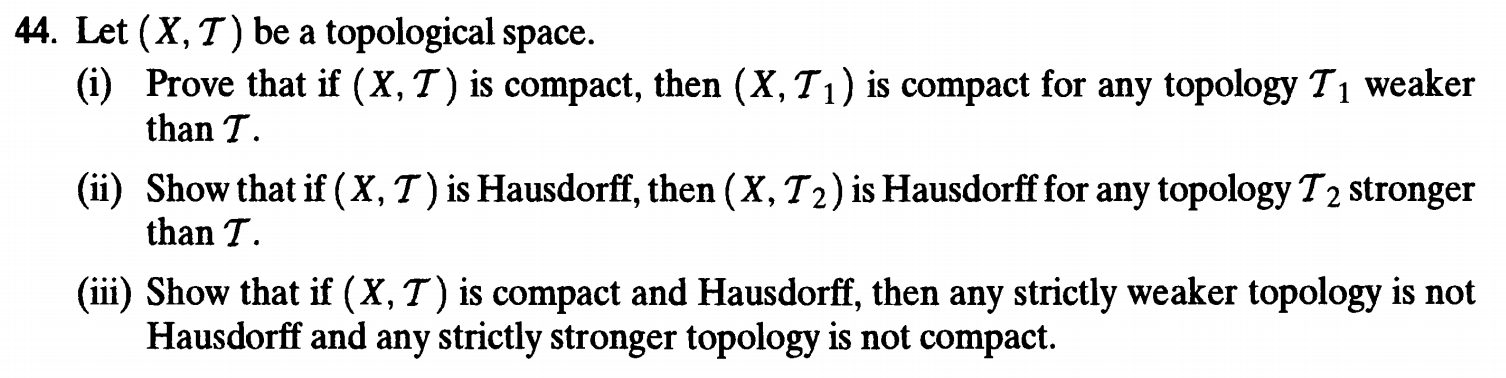
\includegraphics[width=1\textwidth]{11-44}
\end{figure}
\end{question}
\begin{solution} 
Before preceeding to the main problem, we state the following preposition: \\ 
Let $(X,\mathscr{T})$ be a topological space, and $(X,\mathscr{T}_1)$ be
a topological space such that $\mathscr{T}_1$ is weaker or stronger
than $\mathscr{T}$.
Let $E$ be a subset of $X$. Then, the subspace topology of
$\mathscr{T}_1$ on $E$ is still weaker or stronger 
than the subspace topology of $\mathscr{T}$ on $E$. \\
 
By definition of subspace topology, we have
\eQb
\mathscr{T}_{E} = \{ E \cap U \> | \> U \in \mathscr{T} \} \\
{\mathscr{T}_{1}}_{E} = \{ E \cap U \> | \> U \in \mathscr{T}_1 \}. \\
\eQe 
Let $A \in {\mathscr{T}_{1}}_{E}$. Then, $A = E \cap U$ for some $U \in
\mathscr{T}_1$. As $\mathscr{T}_1 \subseteq \mathscr{T}$, $A = E \cap U$,
and $U \in \mathscr{T}$. Hence, $A \in \mathscr{T}_E$. the subpsace topology
of $\mathscr{T}_1$ on $E$ is still weaker than the subspace toplogy 
of $\mathscr{T}_1$ on $E$. The result for stronger relation can be proven
in the same way. 


\textbf{(i)} 
Let $\mathscr{T}_1$ be a topology for $X$, that is weaker than $\mathscr{T}$.
It follows that $\mathscr{T}_1 \subseteq \mathscr{T}$. Let $E$ be
a subset of $X$, and $\{O_\lambda \}_{\lambda \in \Lambda}$ be 
an open cover of $E$ in $(X,\mathscr{T}_1)$. 
As $\mathscr{T}_1 \subseteq \mathscr{T}$, 
the considered open cover is also an open cover in $(X,\mathscr{T})$. 
By compactness of $(X,\mathscr{T})$, 
there exists a finite sub-collection of the open cover, that covers $E$.
Hence, $(X,\mathscr{T}_1)$ is compact. \hfill $\qed$ 

\smallskip

\textbf{(ii)}
Let $\mathscr{T}_2$ be a topology for $X$, that is stronger than 
$\mathscr{T}$. It follows that $\mathscr{T} \subseteq \mathscr{T}_2$. 
If $|X| < 2$, $X$ with any topology is trivially Hausdorff. Hence,
we only consider the remaining case of $|X| \geq 2$. 
Let $x,y \in X$ such that $x \neq y$. As $(X,\mathscr{T})$ is Hausdorff,
there exists a neighborhood of $x$, and a neighborhood of $y$, that are
disjoint, which we denote as $U$ and $V$ respectively. As 
$\mathscr{T} \subseteq \mathscr{T}_2$, $U$ and $V$ are also open in 
$(X,\mathscr{T}_2)$. Hence, $U$ is a neighborhood of $x$, and $V$
is a neighborhood of $y$ in $(X,\mathscr{T}_2)$. Moreover, $U$ and $V$ are
disjoint. Hence, $(X,\mathscr{T}_2)$ is Hausdorff. \hfill $\qed$
 
\smallskip

\textbf{(iii)} 
Let $\mathscr{T}_1$
be a topology for $X$, that is strictly weaker than $\mathscr{T}$. It follows
that there exists a subset $E$ of $X$ such that it is open in 
$(X,\mathscr{T})$, but not open in $(X,\mathscr{T}_1)$. Furthermore, 
$X \setminus E$ is closed in $(X,\mathscr{T})$, but not closed in
$(X\mathscr{T}_1)$. As $(X,\mathscr{T})$ is compact and $X \setminus E$
is closed in $(X,\mathscr{T})$, $(X\setminus E, \mathscr{T}_{X\setminus E})$,
where $\mathscr{T}_{X\setminus E}$ denotes the standard subspace topology 
with respect to $X \setminus E$, is compact. By the stated preposition
on the top, $(X \setminus E , \mathscr{T}_{X \setminus E}$  
is weaker than $(X\setminus E , {\mathscr{T}_1}_{X \setminus E})$. Therefore,
by (i), $(X \setminus E, \mathscr{T_1}_{X \setminus E})$ is compact. 
Suppose for sake of contradiction that $(X, \mathscr{T}_1)$
is Hausdorff. It implies that $X \setminus E$ is closed in
$(X,\mathscr{T})$, which is a contradiction. Hence, $(X,\mathscr{T}_1)$
is not Hausdorff. \hfill $\qed$

\smallskip
 
Let $\mathscr{T}_2$ be a topology for $X$, that is strictly stronger than
$\mathscr{T}$. It follows that there exists a subset $E$ of $X$ such that
it is open in $(X,\mathscr{T}_2)$, but not open in $(X,\mathscr{T})$. 
Furthermore, $X\setminus E$ is closed in $(X,\mathscr{T}_2)$, but not
closed in $(X,\mathscr{T})$. Suppose for sake of contradiction that 
$(X,\mathscr{T}_2)$ is compact. Then, as $X \setminus E$ is closed in
$\mathscr{T}_2$,  
$X\setminus E$ is compact as a subspace topology of $\mathscr{T}_2$ on 
$X \setminus E$. 
As $\mathscr{T}$ is weaker than $\mathscr{T}_2$, by the stated preposition 
on the top, $X \setminus E$ is compact in $(X,\mathscr{T})$. As
$(X\mathscr{T})$ is Hausdorff and compact now, 
$X\setminus E$ is closed in $(X,\mathscr{T})$,
which is a contradiction. Hence, $(X,\mathscr{T}_2)$ is not compact. 
\hfill $\qed$ 
\end{solution}

\bigskip

\begin{question}[4. Royden 11-46]
\hfill
\begin{figure}[h!]
  \centering
    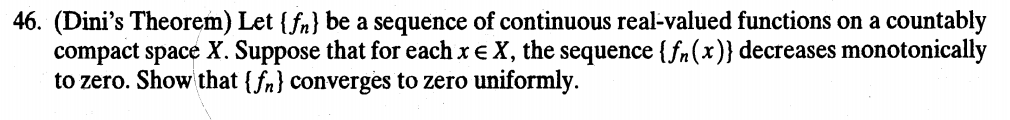
\includegraphics[width=1\textwidth]{11-46}
\end{figure}
\end{question}
\begin{solution}
Fix $\epsilon > 0$.
Define $X_n$ by
\eQb
X_n &=& \{ x \in X \> | \> 
f_n(x) < \epsilon \} ,
\eQe
for all $n \in \mathbb{N}$. As $\{f_n(x)\}$ decreases to 0 monotonically
for all $x \in X$,
we have $\bigcup_{n=1}^{\infty} X_n = X$, and $\{ X_n \}$ is ascending.
Re-writing $X_n$s in terms of pre-images gives  
\eQb
X &=& \bigcup_{n=1}^{\infty} {f_n}^{-1}(B(0,\epsilon )). \\
\eQe
As $f_n$ is continuous for all $n$, each $f_{n}^{-1}(B(0,\epsilon ))$
is open. Therefore, $\{ f_n^{-1}(B(0,\epsilon )) \}$ 
is a countable open cover of $X$. As $X$ is countably compact and, 
there exists a finite subcover of the open cover, yielding
\eQb
X &=& \bigcup_{i=1}^{K} \{{f_{n_i}}^{-1}(B(0,\epsilon )). \\ 
\eQe
Since the pre-images form an ascending collection, we have
\eQb
X &=& f_{n_K}^{-1}(B(0,\epsilon )) \\
&=& \{ x \in X \> | \> f_{n_K}(x) < \epsilon \}. \\
\eQe
Again as $\{f_n(x) \}$ decreases $0$ monotonically for all $x \in X$,
it follows that
\eQb
X &=& \{ x \in X \> | \> f_{j}(x) < \epsilon \> \text{ for } j \geq n_K \}.
\eQe 
Since $\epsilon$ was arbitrary, $\{f_n\}$ converges to $0$ uniformly. 
\hfill $\qed$
 

\end{solution}

\newpage

\begin{question}[4. Royden 12-16]
\hfill \\
\begin{figure}[H]
  \centering
    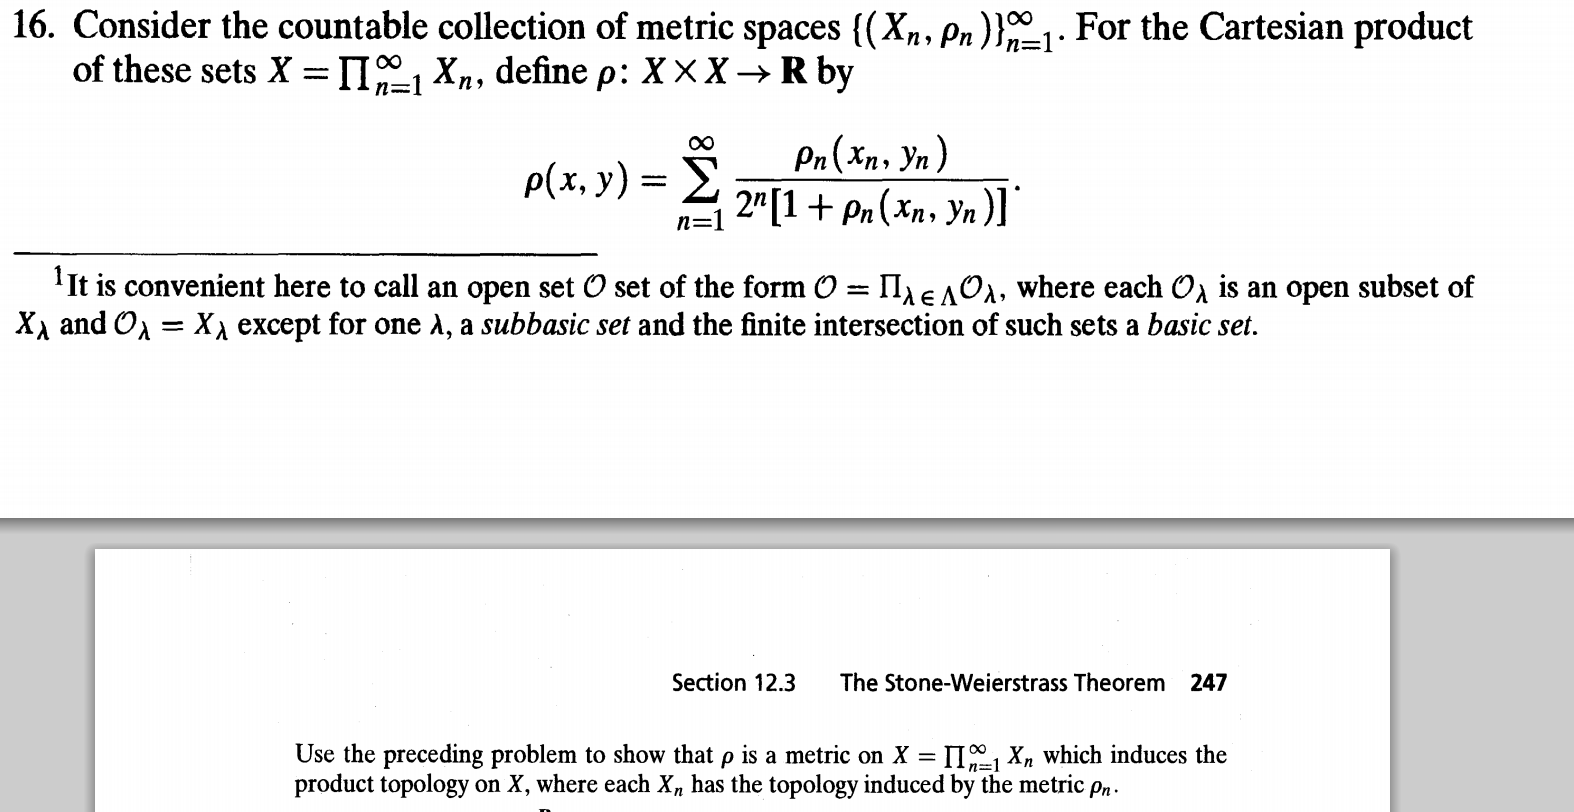
\includegraphics[width=1\textwidth]{12-16}
\end{figure}
\end{question}
\begin{solution}
Let $\mathscr{T}_n$ be the topology on $X_n$, induced by 
the metric $p_n$ on $X_n$. Note that by the problem 15, the
metric ${p_n}^{*}$ on $X_n$,
which is defined by ${p_n}^{*}(x,y) = \dfrac{p(x,y)}{1+p(x,y)}$,
also induce $\mathscr{T}_n$ as well. Let $\mathscr{T}$ be the
product topology defined on $\{ (X_n, T_n )\}$. Let $(X,\mathscr{S})$
be the topological space, induced by the metric space $(X,p)$, which
we have shown indeed to be a metric space in the previous problem set.
We claim that $\mathscr{T} = \mathscr{S}$. We show that for each 
$x \in X$, and for each base $B_{\mathscr{T}}$ of $x$ for $\mathscr{T}$,
there is a base  $B_{\mathscr{S}}$ of $x$ for $\mathscr{S}$, such that
$B_{\mathscr{S}} \subseteq B_{\mathscr{T}}$, and the reverse direction as 
well.

Let $x \in X$.
Let $B_{\mathscr{T}}$ be a base for $\mathscr{T}$. By the definition of
product topology, we can write
\eQb
B_{\mathscr{T}} &=& \prod_{n=1}^{\infty} O_{n},
\eQe
where each $O_n \in T_n$ and $O_n = X_n$ for all but finitely many $n$,
we refer to the finite index set at which $O_n = X_n$ occurs as $F$.
From the previous problem, we have shown that $(\mathscr{T}_n)$ is
also induced by the metric $p^*(x,y) = \dfrac{p(x,y)}{1+p(x,y)}$. Therefore,
for each finitely many $n$ such that $O_n \neq X_n$,
there exists some $\epsilon > 0$, 
$O_n = \{ y_n \in X_n \> | \> \dfrac{1}{2^n} \cdot
\dfrac{p(x_n^*,y_n)}{1+p(x_n^*,y_n)}
< \epsilon_n \}.$ Set $\epsilon = \min_{n \in F}
 \{ \epsilon_n\}$ from the finitely
many $n$s. Consider a base for $\mathscr{S}$ as follows:
\eQb
B_{\mathscr{S}} &=& \{ y \in X| 
\sum_{n=1}^{\infty} \dfrac{p_n(x_n,y_n)}{2^n(1+p_n(x_n,y_n))} < \epsilon 
\text{ and } x_n = x_n^* \text{ for } n \in F; \text{ arbitrary otherwise} \}.
\eQe
Since the sum is less than $\epsilon$ and each distance is non-negative
, it follows that $B_{\mathscr{S}} \subset B_{\mathscr{T}}$.

\smallskip  

Let $x \in X$. Let $B_{\mathscr{S}}$ be a base of $x$ for $\mathscr{S}$. By
the given metric space, we can write
\eQb
B_{\mathscr{S}} = \{ y \in X \> | \> 
\sum_{n=1}^{\infty} \dfrac{p_n(x_n,y_n)}{2^n[1+p_n(x_n,y_n)]} < \epsilon \},
\eQe
for some $\epsilon > 0$. As the series in the metric converges, there exists
$N$ such that $\sum_{n=N}^{\infty} \dfrac{p_n(x_n,y_n)}{2^n[1+p_n(x_n,y_n)]}
< \dfrac{\epsilon}{2}$. Now, consider a base for $\mathscr{T}$ as follows:
\eQb
B_{\mathscr{T}} &=& \prod_{n=1}^{\infty} O_n \\
&\text{where}& \\
O_n &=& B(x_n,\dfrac{\epsilon}{2(N-1)}) \text{ for } n <N \\
O_n &=& X_n \text{ for } n \geq N. \\
\eQe
It follows that for $y \in B_{\mathscr{T}}$,
\eQb
\sum_{n=1}^{\infty} 
\dfrac{p_n(x_n,y_n)}{2^n[1+p_n(x_n,y_n)]} 
&<& (N-1)\dfrac{\epsilon}{2(N-1)} + 
\sum_{n=N}^{\infty}  
\dfrac{p_n(x_n,y_n)}{2^n[1+p_n(x_n,y_n)]} \\
&<& \dfrac{\epsilon}{2} + \dfrac{\epsilon}{2} = \epsilon. 
\eQe
Hence, $B_{\mathscr{T}} \subseteq B_{\mathscr{S}}$. Therefore, $\mathscr{T}
= \mathscr{S}$. \hfill $\qed$
 
\end{solution}

\newpage

\begin{question}[6. Royden 12-20]
\hfill
\begin{figure}[h!]
  \centering
    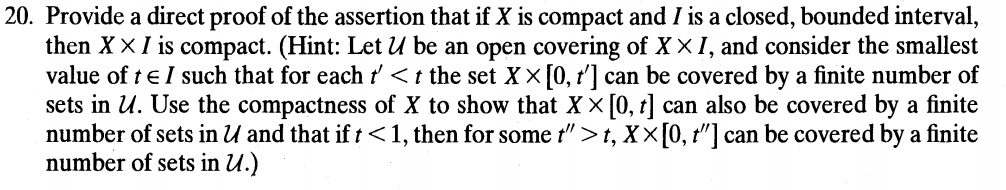
\includegraphics[width=1\textwidth]{12-20}
\end{figure}
\end{question}
\begin{solution}
The direct proof of this problem, which does not appeal to the Tychonoff 
theorem, even the countable case,
will resemble the proof of Heine-Borel theorem in $\mathbb{R}$.
Let $X$ be a compact topological space, and $I$ be a closed, bounded
interval. Consider $X \times I$, which can be written as $X \times [a,b]$.
Let $\mathscr{U}$ be the open cover of $X \times [a,b]$. Define a set $S$
by 
\eQb
S = \{ t \in [a,b] \> | \> X \times [a,t] \> \text{ can be covered 
a finite number of the sets of } \> \mathscr{U} \}. 
\eQe
We first show that $a \in S$, and $S$ is nonempty. Consider $t = a$,
which corresponds to $X \times \{ a \}$. This set is compact, as one can
establish hoemomorphism from $X$ to $X \times \{ a\}$ with the obvious map,
$f(E,a) \to E$, and $X$ compactness is preserved under homeomorphism.
Since $S$ is nonempty, and 
is bounded above by $b$, by the completeness of $\mathbb{R}$, E has 
a supremum. Let $c = \sup S$. Observe that $c \leq b$, as the elements in
$S$ were drawn from $[a,b]$. It thus remains to be shown that $c \geq b$
to show that $c = b$. Suppose for sake of contradiction
that $c < b$. Observe that as $\mathscr{U}$ covers $X \times [a,b]$, 
there exists an open set in the product topology, such that $O_X \times
O_{[a,b]}$ such that $c \in O_{[a,b]}$. From the openness of $O_{[a,b]}$
there exists $\epsilon > 0$, such that  $(c-\epsilon, c+\epsilon)$ is
contained in $O_{[a,b]}$. Hence, $O_X \times (c-\epsilon c+\epsilon)$ is
an open cover of $c$. Now, for the point $c - \dfrac{\epsilon}{c}]$ is 
in $S$. Hence, $[a,c-\dfrac{\epsilon}{2}]$ can be covered by a finite 
subcover of $\mathscr{U}$. Now, the subcover with $O_X \times 
(c-\epsilon, c+ \epsilon)$ covers $[a, c+ \dfrac{\epsilon}{2}]$ and 
contradicts the fact that $c = \sup E$. 
Hence, $c \geq b$ and we have shown that
$c=b$. The exact same line of argument, which will consider the open interval
around $b$ and choosing the finite subcover of an interval with its right 
end-point close enough  will show that $b \in S$. Therefore, we have
shown that $X \times [a,b]$ is compact. 
\hfill $\qed$
\end{solution}


\end{document}
